  \documentclass[xcolor=svgnames]{beamer}
\usepackage[utf8x]{inputenc}
%\usepackage[spanish]{babel}
\usepackage{times}
\usepackage{cite}
\usepackage{xcolor}
\usepackage{multicol}
\usepackage{url}
\usepackage{alltt}
\usepackage{amsthm}
\usepackage{color}
\usepackage{CJK}
\usepackage{enumerate}
\usepackage{listings}
\usepackage{textpos}
\usepackage{fancybox}
\usepackage{eurosym}
\usepackage{graphics,graphicx,color,colortbl}
\usepackage{subfigure}
\usepackage{algorithm}
\usepackage{float}
\usepackage{graphicx}
%\usepackage{subcaption}
\usepackage{subfloat}

\usetheme{Berlin}
\useoutertheme{shadow}
\useoutertheme{split}
\useinnertheme{rounded}
\useoutertheme{infolines}
\usecolortheme{orchid}
\usecolortheme{whale}
\setbeamertemplate{navigation symbols}{}
\setbeamercolor{bgcolor}{fg=black,bg=GhostWhite}
\setbeamercovered{transparent}

\title[Electromagnetic Field Measurement]{Electromagnetic Field Measurement Method to Generate Radiation Map}
\author[David Martínez y Luis Melo]{David Ricardo Martínez Hernández \\ Luis Aníbal Melo Rivera}
\institute[UNAL]{Faculty of Engineer\\ Department of Electric and Electronic \\ National University Of Colombia}
\date[09/28/2012]{September $28$, $2012$}

\begin{document}
\begin{frame}
\titlepage
\end{frame}

\begin{frame}
\frametitle{Table Of Contents}
\tableofcontents
\end{frame}

\section{Introduction}
\begin{frame}
\frametitle{Introduction}
\begin{itemize}
 \item Radio-based technologies bring two factors that must be well managed in order to increase a real quality of life in our society. One of them is the great set of opportunities for social development that these technologies provide and the other is the need of an environmentally friendly technology deployment for anticipating what some people call electrosmog.\pause
 \item Spectrum managements, and standards and regulations for Non-ionizing radiation need to be implemented in each country where wireless telecommunications demand is being increased continuously like in Colombia.
\end{itemize}
\end{frame}

\section[Methodology To Generate Georeferenced Maps]{Methodology To Generate Georeferenced Maps Of Non Ionizing Radiation In A City}
\subsection{Pre-engineering process}
\begin{frame}
\frametitle{Pre-engineering process}
 \begin{itemize}
  \item Segmentation of the city.\pause
  \item Extracting a map of georeferenced antennas in the city.\pause
  \item Definition of measurement routes.\pause
  \item Determination of type of electromagnetic field region.\pause
  \item Determining the field to be measured (electric and/or magnetic).\pause
  \item Selection of equipment and probes for broadband measurement.
 \end{itemize}
\end{frame}

\subsection{Measurement process}
\begin{frame}
\frametitle{Measurement process}
 \begin{itemize}
  \item Automatic taking of broadband measurement.\pause
  \item Frequency selective measurements for hotpoints.\pause
  \item Broadband EMF measurement by route.
 \end{itemize}
\end{frame}

\subsection{Analysis data process}
\begin{frame}
\frametitle{Analysis data process}
 \begin{itemize}
  \item Statistic analyze of measurement.\pause
  \item Performing of continuous radiation map of the city.
 \end{itemize}
\end{frame}

\section{Measurements And Results}
\begin{frame}
 \frametitle{Measurements And Results}
 \begin{table}[H]
	\centering
\begin{tabular}{|c|c|c|}\hline
\textbf{\# Antennas} & \textbf{Service Type} & \textbf{Approximate frequency} \\ \hline
78 & Celular Teleohony & $850$, $900$ $1900$ MHz \\ \hline
12 & Broadcasting on FM & $90\ \ -\ \ 104$ MHz \\ \hline
11 & Broadcasting on AM & $880\ \ -\ \ 1390$ KHz \\ \hline
2 & Trunking System & $800$ Mhz \\ \hline
    \end{tabular}
	\caption{Antennas inventory inside and outside of Bucaramanga city.}
	\label{tab1}
\end{table}
\end{frame}

\begin{frame}
 \begin{figure}[H]
    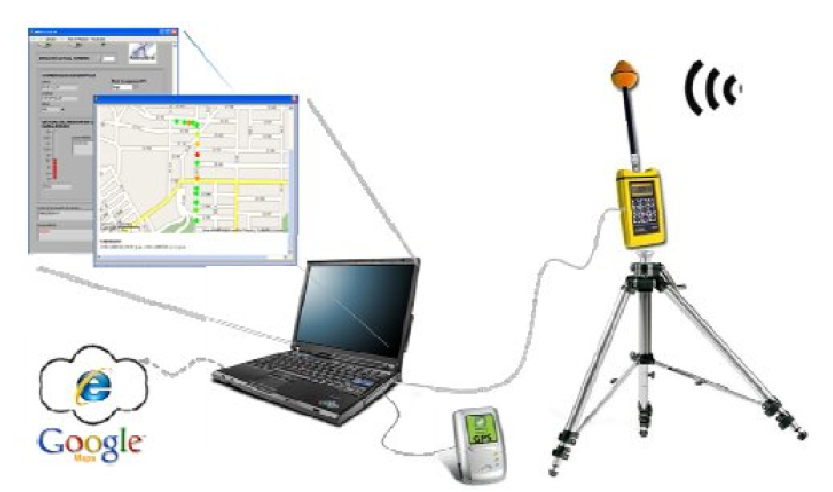
\includegraphics[scale=0.38]{trasns.png}
      \caption{Measurement System\footnote{Copy to Electromagnetic field measurement method to generate radiation map, Page 4}.}
    \end{figure}
\end{frame}

\begin{frame}
 \begin{figure}[H]
    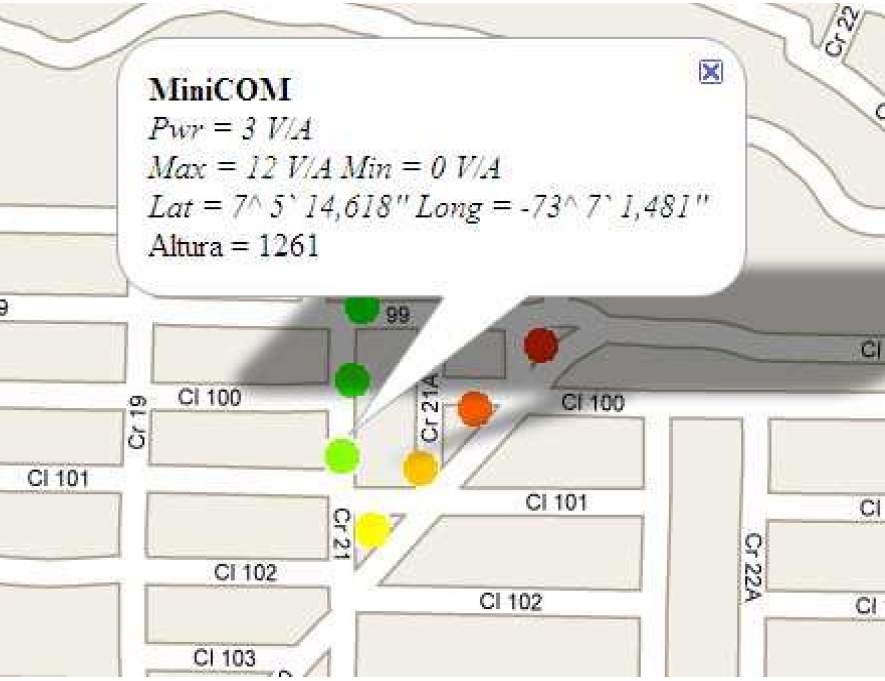
\includegraphics[scale=0.295]{map.png}
      \caption{Map generated by Georadscaner.}
    \end{figure}
\end{frame}

\begin{frame}
 \begin{figure}[H]
    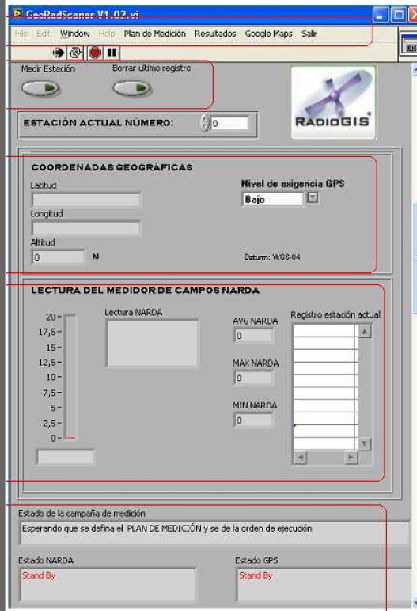
\includegraphics[scale=0.32]{pro.png}
      \caption{Window main Georadscaner.}
    \end{figure}
\end{frame}

\begin{frame}
 \begin{figure}[H]
    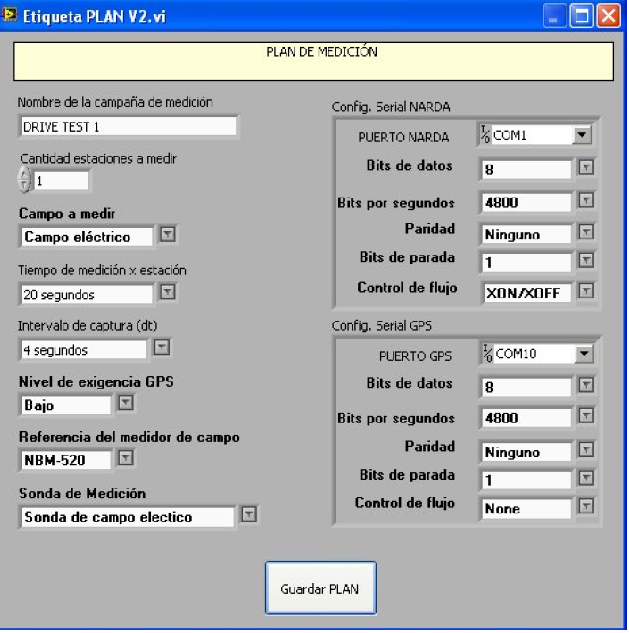
\includegraphics[scale=0.315]{win.png}
      \caption{Window to set the measurement plan.}
    \end{figure}
\end{frame}

\begin{frame}
 \frametitle{Measurements And Results}
 \begin{table}[H]
	\centering
\begin{tabular}{|c|c|c|}\hline
\textbf{Radiation} & \textbf{Range} & \textbf{Description} \\
\textbf{Level} & \textbf{[V/m]} & \\ \hline
Low & 0-0.8 & Residential and educational areas and four \\
 &  & main hospitals. North zone. \\ \hline
Medium & 0.8-2.0 & Business district and shopping areas at old\\
 &  & city (commercial areas). West central, east\\
&  & and south zones. \\ \hline
High & over 2.0 & Specific sites: Court house, city hall and\\
 &  & around 2 important shopping centers. \\ \hline
Hotpoint & over 28 & None \\ \hline
    \end{tabular}
	\caption{Radiation level of Bucaramanga city}
	\label{tab2}
\end{table}
\end{frame}

\begin{frame}
 \begin{figure}[H]
    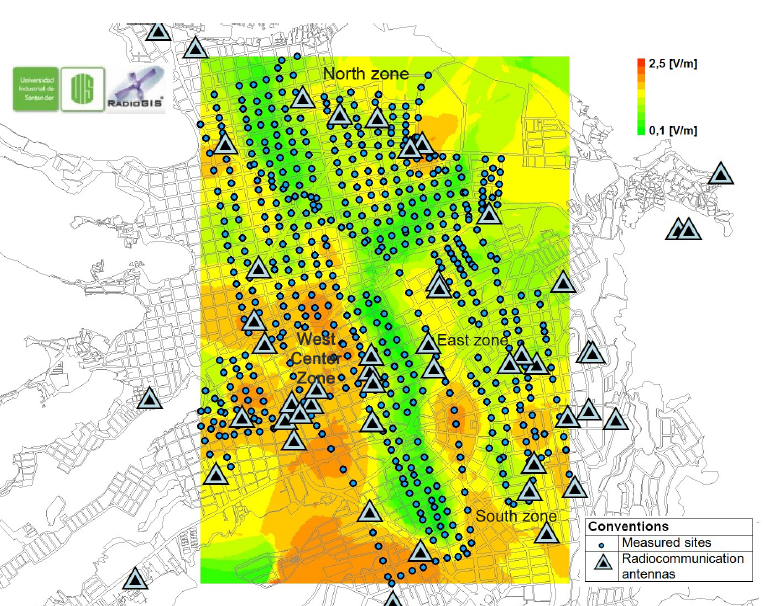
\includegraphics[scale=0.31]{city.png}
      \caption{Map of non-ionizing electromagnetic radiation in Bucaramanga city\footnote{Copy to Electromagnetic field measurement method to generate radiation map, Page 6}}
    \end{figure}
\end{frame}

\section{Conclusions}
\begin{frame}
\frametitle{Conclusions}
\begin{itemize}
 \item A radiation monitoring method was designed and tested during measurement campaigns at city urban zones by covering 70\% of Bucaramanga city area; it was registered around 52 points per Km2 for a total amount of 564 measured points. An iterative and agile process was explained and accomplished into a practical and semi automatic way to record field strength of electromagnetic waves by using both broadband field meter and spectrum analyzer in order to establish whether regulation norms are being met and to know which factors are contributing to radiation level increasing by means of a spectral view. Also a telecommunications service was developed to measure, send and request online for measured data in real time and integrated into a Geographic Information System supported by RadioGis R\&D Group with a web platform of Telecommunication services.
\end{itemize}
\end{frame}

\section{Bibliography}
\begin{frame}
\frametitle{Bibliography}
\begin{thebibliography}{10}

\bibitem{conference} \textbf{Conference Publications:} Volcanic Environments Robots for exploration and Measurement By  Rodriguez, C.C. Grupo de Investig. RadioGIS, Univ. Ind. de Santander, Bucaramanga, Colombia Forero, C.A. ;  Boada, H.O.. Date of Conference: 16-18 May 2012.

\bibitem{page} Web Site: \url{http://ieeexplore.ieee.org/xpl/mostRecentIssue.jsp?punumber=6225461}

\end{thebibliography}
\end{frame}
\end{document}